    \documentclass[12pt, twoside, notitlepage, twocolumn]{article}
    \setlength{\columnsep}{0.5cm}
    \usepackage[a4paper, left=0.5cm,right=0.5cm,top=0cm,bottom=0.5cm]{geometry}
    \usepackage{amsmath,bm}
    \usepackage{sectsty}
    \usepackage{graphicx}
    \usepackage{tabularx}
    \usepackage{hyperref}
    \sectionfont{\fontsize{12}{12}\selectfont}
    \setlength{\parindent}{0pt}

    \newcommand{\makeabs}
    {
        \textbf{Abstract:}
        A set of selected $p p$ collision data samples which were collected by LHCb\cite{1748-0221-3-08-S08005} in 2011 are studied.
        Contained $B^{\pm}\rightarrow\pi^{\pm}\pi^{+}\pi^{-}$ decays in magnet ``up'' and ``down'' 
        polarity are constructed. Global $CP$ asymmetry in this channal is measured to be 
        $A_{CP}=0.126\pm0.023\pm0.026$,
        in which the first and second uncertainties are statistical and systematical respectively. 
        Larger local asymmetry in different phasespace is also observed.
        \newline\hbox{}
    }

    \newcommand{\makeauth}
    {
        Qichen Dong, Harriet Watson\newline
        School of Physics and Astronomy, University of Manchester, Manchester, M13 9PL.
    }
    \newcommand{\maketit} 
    {
        \textbf{Measurement of $\bm{CP}$ Violation in $\bm{B^{\pm}\rightarrow\pi^{\pm}\pi^{+}\pi^{-}}$ 
        Decay Channal at Large Hadron Collider}
    }
% Document begins
    \begin{document}
        \twocolumn[\begin{@twocolumnfalse}
            \begin{flushleft}
                \maketit
                \makeauth
            \end{flushleft}
            \makeabs
        \end{@twocolumnfalse}]

        \section{Introduction}
        The Standard Model\cite{1412.4094} (SM) of particle physics, which developed in early 1970s, has been successfully 
        explaining almost all experiment results and made precise predictions including Higgs boson before 
        it was discovered. Although the SM has been considered as the best theory describing 
        fundamental particles and their interaction, phenomena such as large scale of matter antimatter 
        asymmetry in the universe are not fully explained. Matter antimatter asymmetry is described by Charge
        Parity (CP) invarinace violation in the SM, but the effect is too small to explain the reason 
        why objects in the universe is made almost entirely of matter, while only small amount of antimatter 
        managed to survive. Therefore, additional sources of CP violation from new physics above SM
        may contributes to the exceeding magnitude of asymmetry. Charmless B meson to 3 hadrons decay is observed 
        to have the largest CP violation, also contains rich interference pattern gives us a chance to investigate 
        the asymmetry originate from different resonant states in the phase space.\cite{1310.4740} Measuring CP 
        violation provides evidence of physics beyond Standard Model.
        \section{Candidates Selection}
        The LHCb\cite{1748-0221-3-08-S08005} detector is designed for studying particles containing $b$ and $c$ quark.
        Analysed data was preselected by hardware and software trigger from approximatly $10^{14}$ $pp$ collision 
        events with centre-of-mass energy of 7 TeV. Most important pre-selection cuts are listed in the labscript\cite{Labsc}.
        \newline Information from the particle identification system\cite{1211.6759} are used to seperate
        $B^{\pm}\rightarrow\pi^{\pm}\pi^{+}\pi^{-}$ events, apart from rejecting muon, the probability of each 
        particle to be a pion is required to be larger than 0.794, in order to make sure 50 per cent of final decay 
        products are all pion. CP Asymmetry introduced by charmed decay of B mesons are removed by rejecting $D^0$ 
        resonance by excluding $\pm 50MeV$ region of $D^0$ meson invariance mass in two body invariant mass 
        $M_{\pi^+\pi^-}$ phase space. 
        \section{Global Asymmetry}
        Raw asymmetry of $B^{\pm}\rightarrow\pi^{\pm}\pi^{+}\pi^{-}$ modes is defined as $A_{raw} = \epsilon^--\epsilon^+$, 
        where $\epsilon^\pm = \frac{N_{B^\pm}}{N_{B^+}+N_{B^-}}$ is called efficiency. $N_{B^\pm}$ is estemated by fitting $B$ 
        meson invariant mass spectra then integrating signal model contribution. Cruijff function with zero right radiative 
        tail was chosen to be signal model, the mean, width and left tail were left free. We described the combinatorial 
        background by an exponential function, all of its parameters were left to be fitted. Backgrounds caused by four-body-decay 
        were parametrized by gaussian, whose peak positions were fixed to 5134 MeV for $B^+$ and 5040 MeV for $B^-$ by optimizing 
        deduced $\chi^2$ of fitting,  We also tried to introduce a small peak centred in 5215 MeV to describe 
        $B^{\pm}\rightarrow K^{\pm}\pi^{+}\pi^{-}$ in which one Kaon was misidentified, however, contribution of it is negligible 
        with rather strict selection criteria we implemented. The invariant mass contribution and fitting results are shown in figure 1.
        \begin{figure}[!hb]
            \begin{centering}
            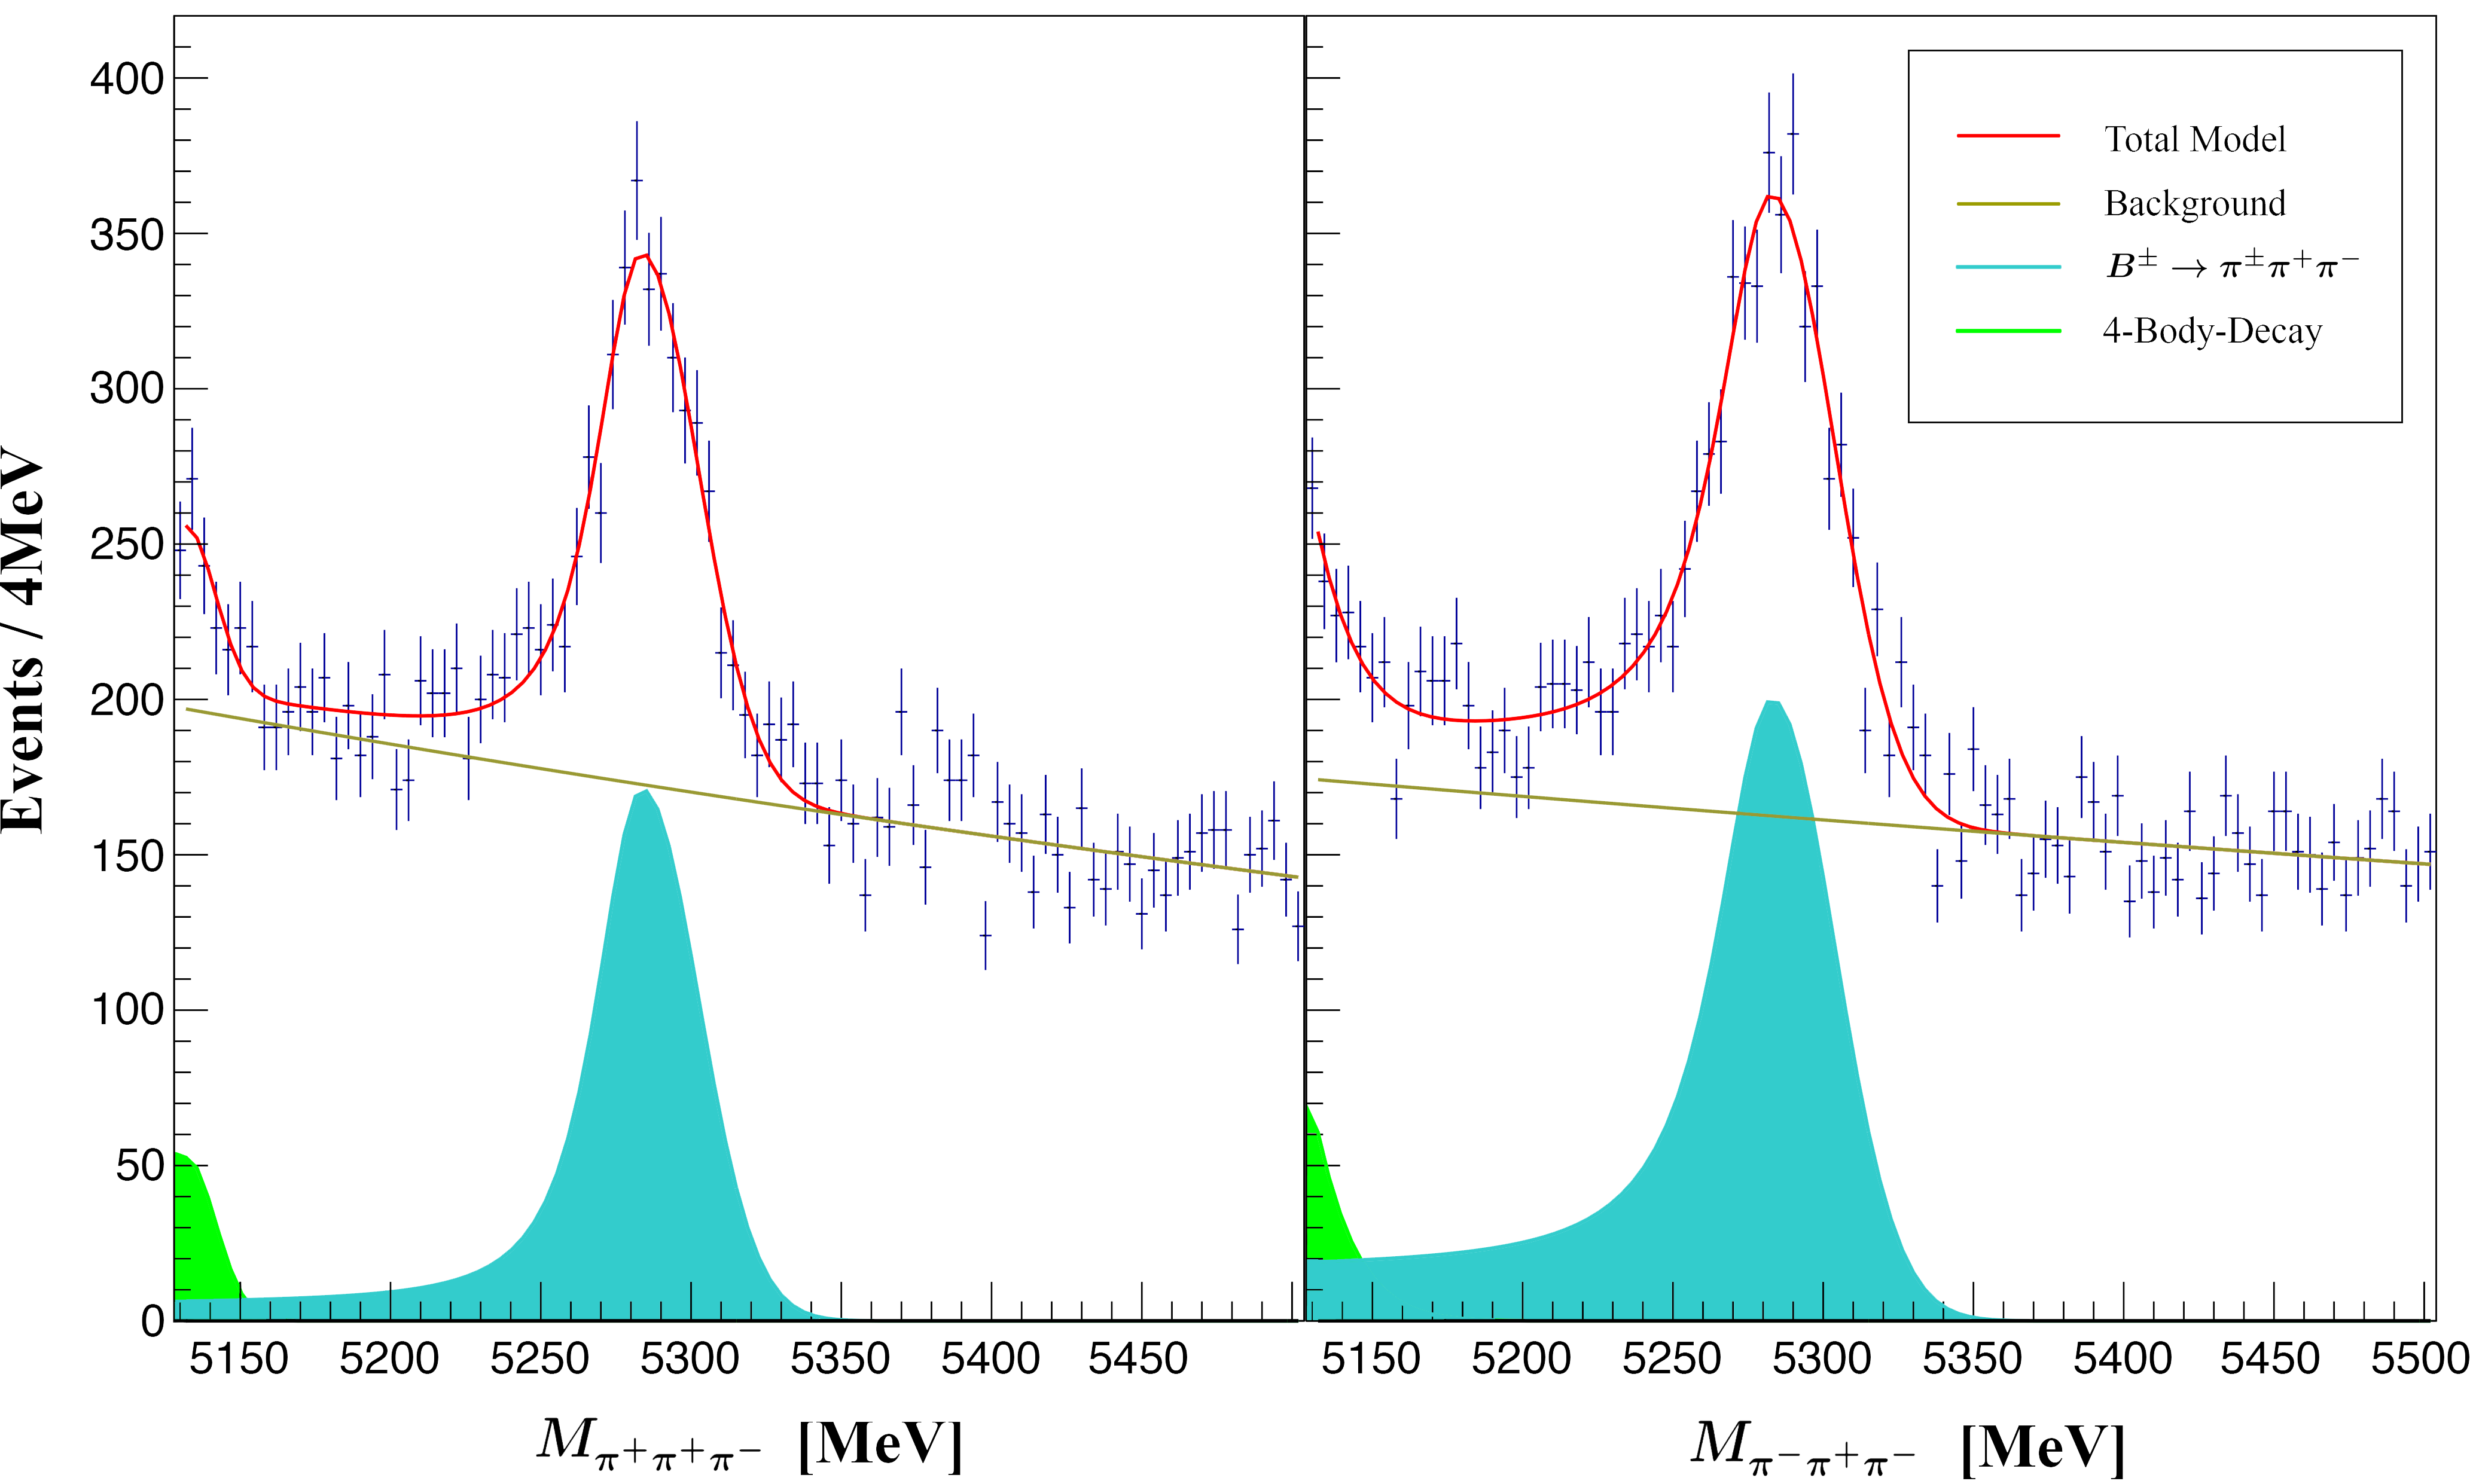
\includegraphics[scale=0.276]{GA.png}
            \caption{Invariant mass spectra and fitting results. \newline Left panel is $B^+$ and Right panel is $B^-$}
            \end{centering}
            \label{fig:label1}
        \end{figure}
        Integral of signal model gives $N_{B^+} = 2251 \pm 81$ and $N_{B^-} = 2789 \pm 82$. Raw CP asymmetry yields $A_{raw}=0.107 
        \pm 0.023 (statistical)$. Since detector efficiencies for $B^+$ and $B^-$ are not equal in different polarities, a detector 
        polarity correction is made based on $\epsilon^\pm_{up}$ and $\epsilon^\pm_{down}$ in two subsets of data, defined as 
        $A_{cor}=\epsilon_{cor}^--\epsilon_{cor}^+$, where $\epsilon_{cor}^\pm = (\epsilon^\pm_{up}+\epsilon^\pm_{down})/2$.
        $A_{CP}$ is constructed by excluding B-meson production asymmetry $A_P = 0.004\pm0.004$\cite{1310.4740} from $A_{cor}$, which 
        yields $A_{CP} = A_{cor} - A_P = 0.126 \pm 0.023$, Uncertainty above is statistical only, estimated by integrating 
        fitting-error within 3-sigma width around signal mean. 4 aspect of sources of systematic uncertainties were studied. uncertainty 
        introduced by polarity correction is significantly larger than other sources, estimated by $\pm(A_{raw}-A_{cor})$.Method used in 
        calculating error of chosen signal model is comparing $A_{raw}$ given by ``similar-good-fitting'' Cruijff function and double 
        gaussian signal model,defined as $\pm(A_{raw}^{Cruijff}-A_{raw}^{Gaussian})$. This two function give deduced $\chi^2_+=1.109,\ 
        \chi^2_-=1.065$ and $\chi^2_+=1.162,\ \chi^2_-=1.118$ respectively. Lorentz function was not included since it gives relatively 
        higher deduced $\chi^2$. By shifting the position of 4-body gaussian funtion, we estimated uncertainty of partially reconstructed 
        4-body-decay. However, its magnitude is around $10^{-5}$, which is negligible. B meson production uncertainty was considered as 
        systematic error. total systematical uncertainty is calculated by sum in quadrature of each contribution, main systemetical 
        uncertainties are listed in Table 1.
        \begin{table}[ht]
            \centering
            \caption{Main systematical Uncertainties}
            \begin{tabularx}{9.73cm}{lXr}
            \hline
            Source & & Uncertainty \\
            \hline
            Polarity Correction  & & 0.023 \\
            Signal Function  & & 0.011 \\
            4-body Backgrounds & & 0.000 \\
            $A_P$ & & 0.004 \\
            \hline
            Total & & 0.026 \\
            \hline
            \end{tabularx}
        \end{table}
        \newline In summary, inclusive CP asymmetry is measured to be $A_{CP} = 0.126\pm0.023(statistical)\pm0.026(systematical)$
        total uncertainty is calculated by $\pm \sqrt{0.023^2+0.026^2}=\pm 0.0347$, significance yeilds $3.63\sigma$.
        \section{Local Asymmetry}
        In order to identify the distribution of CP violation, we studied 
        \section{Conclusions}
        \bibliography{biblio.bib}
        \bibliographystyle{hunsrt}
    \end{document}
